% ============================================================
% IE UNIVERSITY - BAM - ML & Communication Skills Progress Report
% ============================================================

\documentclass[clean]{bam-proposal}

\BAMdeliverable{Progress Report}
\BAMtitle{Early Collision Risk Forecasting from ESA Conjunction Data Messages}
\BAMteam{Pedro Jon Fuentes Garc\'es; Mario Fern\'andez Velasco}
\BAMcourse{Machine Learning \& Communication Skills}
\BAMacademicyear{2026--2027}
\BAMsubmissiondate{1 November 2026}

\BAMbibliographystyle{plainnat}
\BAMbibliographyfile{references}

\begin{document}
\makeproposalheader

\section{Introduction}

Our goal is unchanged since the proposal: using only Conjunction Data Messages (CDMs) received at least two days before the time of closest approach (TCA), we ask which modelling approach improves on the latest-risk prediction (LRP) baseline under the rare-event metrics of the ESA Kelvins challenge, \(F_2\), \(\mathrm{MSE}_{\mathrm{HR}}\) and \(L=\mathrm{MSE}_{\mathrm{HR}}/F_2\)~\citep{uriot2021collision}, and whether a calibrated two-stage design better characterises events whose risk jumps close to TCA. Because LRP is hard to beat~\citep{uriot2021collision}, most of our work so far has gone into fixing what exactly is predicted, from which messages, on which events, and how a comparison is judged. The first models trained under this protocol are still weak: none beats LRP yet. We see them as a baseline for our own pipeline, and the implementation of every model family will keep improving in the coming weeks.

\section{Data and Evaluation Protocol}

We use the public Kelvins training set (13{,}154 events)~\citep{zenodo4463683}. The label of an event is the risk of its last CDM (log\(_{10}\)); an event is high-risk (HR) if that value is at least \(-6\). Inputs are restricted to CDMs with time-to-TCA \(\ge 2\) days (Fig.~\ref{fig:timeline}). This rule exposed an issue the proposal did not anticipate: in 3{,}032 events the last CDM itself lies two or more days before TCA, so the label is also an input and LRP reproduces it exactly. These events hold 71\% of all HR events in the training data. We excluded them, together with events that have no usable CDM, which leaves 8{,}892 events and only 93 HR (1.05\%, against 6.9\% in the official test). We keep the 599 events whose last CDM arrives one to two days before TCA; they are easier for LRP, so validation is somewhat optimistic.

All model comparisons use the same internal protocol: event-level 5-fold cross-validation stratified on the HR label, repeated five times with fixed seeds, with out-of-fold predictions and metrics averaged over repetitions. Uncertainty is estimated with an event-level bootstrap (\(B=10{,}000\), 95\% BCa intervals). The official test set is reserved for a single final evaluation and is used here only to report the baselines already shown in the proposal (Table~\ref{tab:official}). From the exploratory analysis we retain only the extreme imbalance and the frequency of large final risk changes (Fig.~\ref{fig:imbalance}).

\section{Methods}

\textbf{Features.} Each event is one row of 35 features from usable CDMs only: risk, miss distance, relative speed and an orbit-determination quality indicator at the first, last and three intermediate messages; risk minimum, maximum, range, mean and standard deviation; message counts and timing; and object type. The mission identifier is excluded to avoid mission-specific shortcuts.

\textbf{Jump taxonomy.} For analysis only (never as input or target), each event is labelled \emph{stable-low}, \emph{stable-high}, \emph{jump-up} or \emph{jump-down} from the change between last usable and final risk, with a symmetric cut of one order of magnitude, to select and explain failure cases.

\textbf{Course models.} Ordinary least squares, ridge and lasso regress the final log-risk on standardised features. Regularisation strength is chosen by nested cross-validation inside each training fold. Their continuous predictions almost never reach \(-6\), so each model uses an alarm threshold chosen on the training fold to maximise \(F_2\).

\textbf{Tree ensembles.} A random forest and a gradient-boosting regressor (ahead of the syllabus, studied before implementation) regress the same target, with the number of trees selected by out-of-fold \(L\). The first runs gave \(F_2=0\): about 80\% of events sit at the \(-30\) floor of the risk scale, so leaf means never reach \(-6\). We therefore train on the target floored at a value \(c\approx-6.09\), derived in each training fold from the \(F_2\)-optimal decision threshold~\citep{lipton2014optimal}; evaluation still uses the original labels and the fixed \(-6\) alarm line.

\section{Preliminary Results}

No model beats LRP on \(L\) (Table~\ref{tab:internal}). Lasso matches LRP on \(F_2\) (paired difference \(-0.006\), 95\% CI \([-0.057, 0.034]\)), but its error on HR events is far larger, so its \(L\) is more than four times higher. The tree ensembles have the lowest \(L\) among learned models but remain more than three times above LRP. Both trees rely mainly on summaries of the risk history (Fig.~\ref{fig:importance}); geometry and object type contribute little. Two pre-registered checks fired (importance rankings disagree on order; one target-floor criterion for the random forest); neither changes this conclusion, and both are reopened next cycle.

\begin{table}[htbp]
  \small
  \begin{minipage}[t]{0.37\linewidth}
    \centering
    \caption{Official test set (\(n=2167\), 150 HR), baselines as in the proposal.}
    \label{tab:official}
    \begin{tabular}{@{}lccc@{}}
      \toprule
      & \(F_2\) & \(\mathrm{MSE}_{\mathrm{HR}}\) & \(L\) \\
      \midrule
      CRP & 0.271 & 0.679 & 2.504 \\
      LRP & 0.739 & 0.513 & 0.694 \\
      \bottomrule
    \end{tabular}
  \end{minipage}\hfill
  \begin{minipage}[t]{0.60\linewidth}
    \centering
    \caption{Internal protocol (8{,}892 events, 93 HR), out-of-fold means of five repeated 5-fold CVs; brackets: 95\% BCa bootstrap. Preliminary.}
    \label{tab:internal}
    \begin{tabular}{@{}lll@{}}
      \toprule
      Model & \(F_2\) & \(L\) \\
      \midrule
      LRP & 0.492 & 0.548 \\
      OLS\(^{a}\) & 0.264 \([0.216, 0.317]\) & 4.41 \([3.23, 6.35]\) \\
      Ridge\(^{a}\) & 0.284 \([0.234, 0.336]\) & 4.11 \([3.03, 5.88]\) \\
      Lasso\(^{a}\) & 0.486 \([0.413, 0.557]\) & 2.40 \([1.80, 3.45]\) \\
      Random forest\(^{b}\) & 0.433 & 1.87 \\
      Gradient boosting & 0.417 & 1.87 \\
      \bottomrule
    \end{tabular}
  \end{minipage}

  \smallskip
  {\footnotesize \(F_2\) higher is better; \(\mathrm{MSE}_{\mathrm{HR}}\) and \(L\) lower are better; \(L\) uses \(\mathrm{MSE}_{\mathrm{HR}}\) clipped at \(-6.001\).
  \(^{a}\)Alarm threshold chosen on each training fold to maximise \(F_2\); LRP and the trees alarm at the fixed HR line \(-6\), so \(F_2\) is not computed under the same rule for all rows.
  \(^{b}\)A pre-registered revocation criterion for the training-target floor fired; the floor is re-derived in the next cycle.\par}
\end{table}

\section{Discussion and Next Steps}

The main change since the proposal is methodological. The proposal only scored LRP on the official test; we now compare every model on the same events and folds, and building that protocol forced decisions the proposal did not foresee: excluding events whose label is already an input, a training-target floor for trees, and a per-fold alarm threshold for linear regressors. They also explain why internal LRP (\(F_2=0.49\)) differs from the official test (\(F_2=0.74\)): different events, lower HR prevalence, and most HR events in the excluded group. All model numbers above are preliminary. Next steps: (1) the calibrated two-stage model with a reliability diagram; (2) the failure atlas, with cases chosen from out-of-fold predictions by pre-defined rules; (3) resolving the two open checks and comparable uncertainty for all models; (4) near-final results for the Sentence Outline.

\section*{Declaration of Contributions and AI Use}

We follow a work plan designed together at the start that splits the project into scopes of equal expected effort: Pedro leads protocol, features and trees; Mario leads exploratory analysis, jump taxonomy and course models. Later deliverables will detail individual contributions. Every modelling choice (over fifty so far) is recorded in the repository with the deciding member's own justification, after checking that he understands the method; code may only use registered parameters, and an audit checks this. Pedro used Cursor and Mario used Claude to present options and to write and test code; neither assistant chose a modelling setting.

\BAMprintbibliography

\clearpage
\section*{Figures}

\begin{center}
  \captionsetup{hypcap=false}
  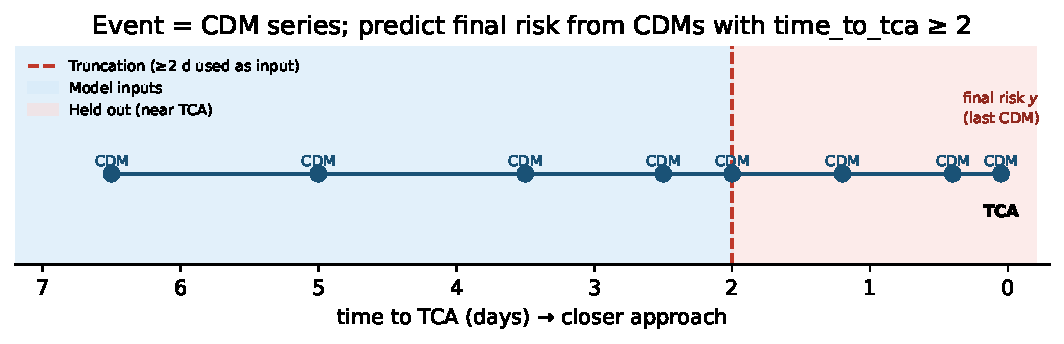
\includegraphics[width=0.68\linewidth]{figures/fig_cdm_timeline.pdf}
  \captionof{figure}{Schematic event (reused from the proposal). Inputs use only CDMs with time-to-TCA \(\ge 2\) days; the label is the risk of the last CDM.}
  \label{fig:timeline}

  \medskip
  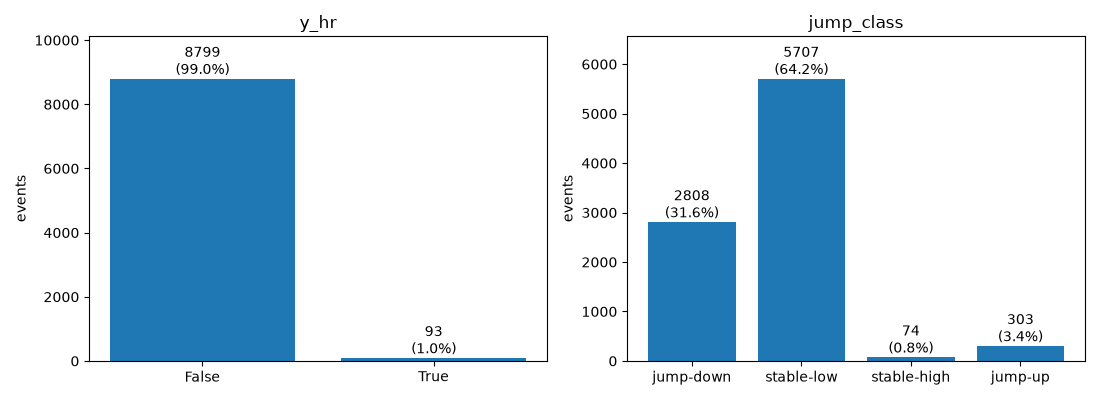
\includegraphics[width=0.85\linewidth]{figures/fig_imbalance_jumps.png}
  \captionof{figure}{Internal event set (8{,}892 events). Left: HR label (True = final risk \(\ge -6\)). Right: jump taxonomy with a cut of one order of magnitude between the last usable risk and the final risk; analysis only, never a model input.}
  \label{fig:imbalance}

  \medskip
  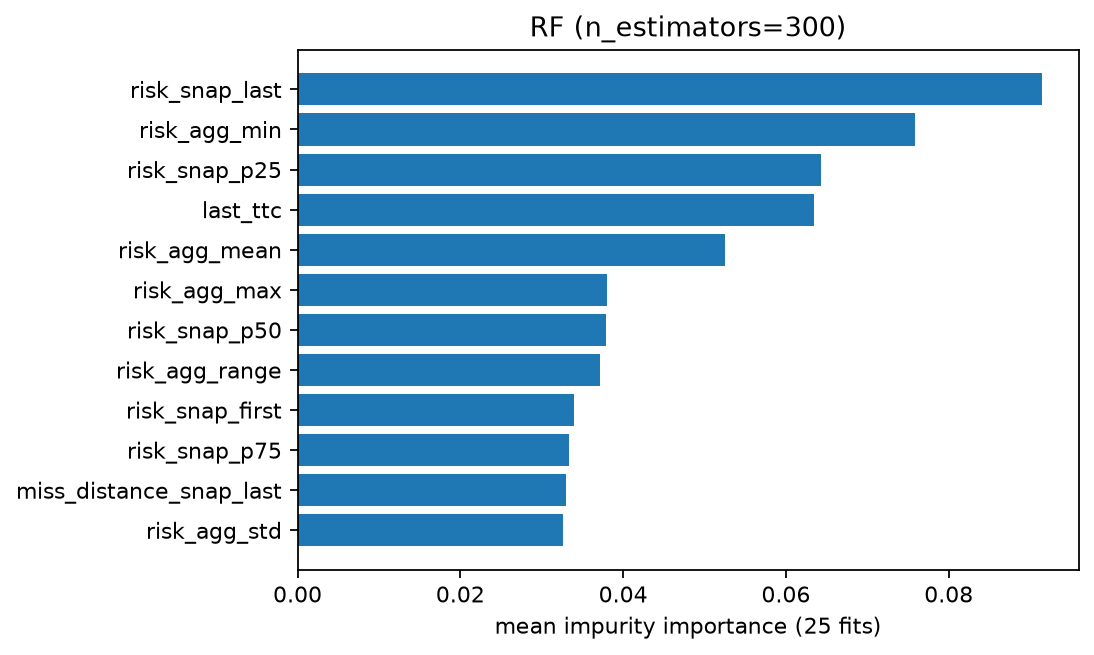
\includegraphics[width=0.60\linewidth]{figures/fig_importance_rf.png}
  \captionof{figure}{Random forest impurity importances averaged over 25 fold fits (top 12). Not causal. Permutation importance on one validation fold agrees that risk summaries dominate but orders them differently (e.g.\ minimum risk first), so no single ranking is claimed.}
  \label{fig:importance}
\end{center}

\end{document}
